\documentclass[english,14pt]{beamer}
\usetheme{EastLansing}
\usecolortheme{spruce}

\usepackage{xcolor}
\usepackage{listings}
\usepackage{courier}
\usepackage{graphicx}
\usepackage{amsmath}
\usepackage{algorithm2e}
\usepackage{multicol}
\usepackage{hyperref}
\usepackage{textcomp}

% http://mirrors.ibiblio.org/CTAN/macros/latex/contrib/datetime2/datetime2.pdf
\usepackage{babel}
\usepackage[useregional]{datetime2}

% https://tex.stackexchange.com/questions/42619/x-mark-to-match-checkmark
\usepackage{pifont}% http://ctan.org/pkg/pifont

%% https://stackoverflow.com/questions/1435837/how-to-remove-footers-of-latex-beamer-templates
%%gets rid of bottom navigation bars
%\setbeamertemplate{footline}[page number]
%
%gets rid of navigation symbols
\setbeamertemplate{navigation symbols}{}


\usefonttheme[onlymath]{serif}

\definecolor{mGreen}{rgb}{0,0.6,0}
\definecolor{mGray}{rgb}{0.5,0.5,0.5}
\definecolor{mPurple}{rgb}{0.8,0,0.82}
\definecolor{backgroundColour}{rgb}{0.95,0.95,0.92}
\definecolor{lightBlue}{rgb}{0.1, 0.1, 0.8}

\newcommand\red[1]{{\color{red} #1}}
\newcommand\green[1]{{\color{green} #1}}
\newcommand\blue[1]{{\color{blue} #1}}

\newcommand{\cmark}{\ding{51}}%
\newcommand{\xmark}{\ding{55}}%

\lstdefinestyle{CStyle}{
    backgroundcolor=\color{backgroundColour},   
    commentstyle=\color{mGreen},
    keywordstyle=\color{magenta},
    numberstyle=\tiny\color{mGray},
    stringstyle=\color{mPurple},
    basicstyle=\footnotesize,
    breakatwhitespace=false,         
    breaklines=true,                 
    captionpos=b,                    
    keepspaces=true,                 
    numbers=left,                    
    numbersep=5pt,                  
    showspaces=false,                
    showstringspaces=false,
    showtabs=false,                  
    tabsize=2,
    language=Python
}

\lstdefinestyle{pseudo}{
        basicstyle=\ttfamily\footnotesize,
        keywordstyle=\color{lightBlue},
        morekeywords={BEGIN,END,IF,ELSE,ENDIF,ELSEIF,PRINT,WHILE,RETURN,ENDWHILE,DO,FOR,TO,IN,ENDFOR,BREAK,INPUT},
        morecomment=[l]{//},
        commentstyle=\color{mGreen}
}

\lstset{basicstyle=\footnotesize\ttfamily,breaklines=true}
\lstset{framextopmargin=50pt,tabsize=2}

\title{ENGG1003 - Monday Week 6}
\subtitle{Interpolation, Assignment 1 and Mid-term quiz}
\author{Steve Weller}
\institute{University of Newcastle}
%\date{\today}
\date{29 March 2021}

% following is a bit of a hack, but forces page numbers (technically: frame numbers) to run 1,2,3,... 
% with titlepage counting as frame 1

\addtocounter{framenumber}{1}
\titlepage

\begin{document}

\begin{flushleft}
{\scriptsize Last compiled:~\DTMnow}
\vspace*{-5mm}
\end{flushleft}
\framebreak

%==============================================================

\begin{frame}[fragile]

\frametitle{Lecture overview}
\begin{enumerate}
	\item Interpolation
	\item[]
	
	\item Assignment 1
	
	\item[]
	
	\item Mid-term quiz

\end{enumerate}

\end{frame}

%==============================================================

\begin{frame}[fragile]

\frametitle{The story so far}
\vspace*{-5mm}
\begin{itemize}
	\item variables and data types
	\item arrays (using \texttt{numpy})
	\item plotting (using \texttt{matplotlib})
	\item flow control
	\begin{itemize}
		\item \texttt{if}
		\item \texttt{while}
		\item \texttt{for}
	\end{itemize}
	\item functions
\end{itemize}
\vspace*{3mm}
Most of ENGG1003 from here uses these elements of Python to solve Engineering problems

\end{frame}

%==============================================================

\begin{frame}[fragile]

\frametitle{$1)$ Interpolation}

Two common forms of \red{\emph{curve-fitting}} in Engineering applications:

\begin{enumerate}
	\item \red{\emph{interpolation}}
	\begin{itemize}
		\item today's lecture
	\end{itemize}
	\item[]
	\item \red{\emph{regression}}
	\begin{itemize}
		\item considered in detail later in ENGG1003
	\end{itemize}
\end{enumerate}
	
\begin{itemize}
	\item we now demonstrate both curve-fitting methods applied to the same dataset
\end{itemize}

\end{frame}

%==============================================================

\begin{frame}[fragile]

\frametitle{Curve-fitting dataset}

\texttt{Week6Mon.py}
\vspace*{-3mm}
\begin{figure}[ht]
	\centering
	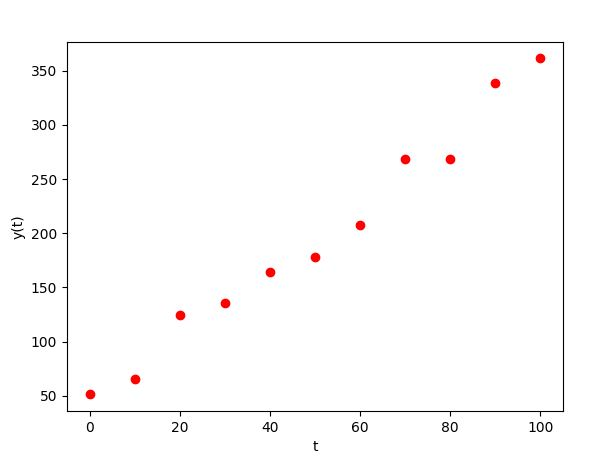
\includegraphics[width=0.6\textwidth]{figures/Week6MonDataset}
\end{figure}
\vspace*{-5mm}
\begin{itemize}
	\item 11 pairs of data points $(t_i,y_i), i = 0,1,2,\ldots,10$
	\item[] {\small $(0,51.29), (10,65.24), (20,124.89), \ldots,(100,361.32)$}
\end{itemize}

\end{frame}

%==============================================================

\begin{frame}[fragile]

\frametitle{Interpolation}

\vspace*{-3mm}
\begin{figure}[ht]
	\centering
	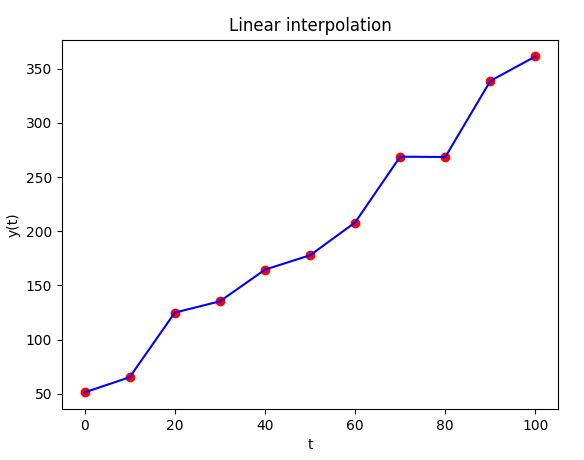
\includegraphics[width=0.8\textwidth]{figures/Week6MonLinearInterp}
\end{figure}

\end{frame}

%==============================================================

\begin{frame}[fragile]

\frametitle{Regression}

\vspace*{-3mm}
\begin{figure}[ht]
	\centering
	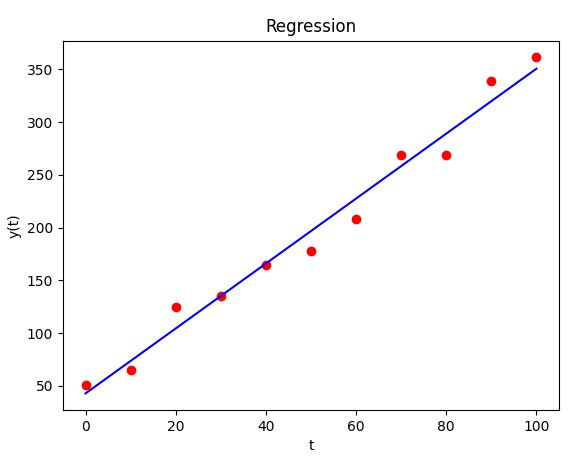
\includegraphics[width=0.8\textwidth]{figures/Week6MonLinearRegression}
\end{figure}

\end{frame}

%==============================================================

\begin{frame}[fragile]

\frametitle{Interpolation vs.\ regression}

\begin{itemize}
	\item \textbf{interpolation:} joining the dots
	\begin{itemize}
		\item obtain value of $y$ at some intermediate point
	\end{itemize}
	\item[]
	\item \textbf{regression:} fitting a straight line
	\begin{itemize}
		\item when there's ``too much data'', simplify
		\item here, simplifying to a straight line
		\item we return to choosing ``best'' straight line later in ENGG1003
		\item no more regression in this lecture
%		\item obtain a ``functional form'' eg: identify a model, F=kx for Hookes' law
	\end{itemize}
	\item[]
	\item both interpolation \& regression involve creating a function \blue{(blue line)} from data \red{(red dots)}
%	\begin{itemize}
%		\item that requires some explanation! so let's do that
%	\end{itemize}
\end{itemize}

\end{frame}

%==============================================================

\begin{frame}[fragile]

\frametitle{Functions}

\begin{itemize}

	\item review mathematical functions: week 5 Monday lecture, page 3
	\item function $f$ takes data point $t$ and returns $y = f(t)$
%	\item review in PyCharm
\end{itemize}

\end{frame}

%==============================================================

\begin{frame}[fragile]

\frametitle{The interpolation problem}

\vspace*{-5mm}
\begin{figure}[ht]
	\centering
	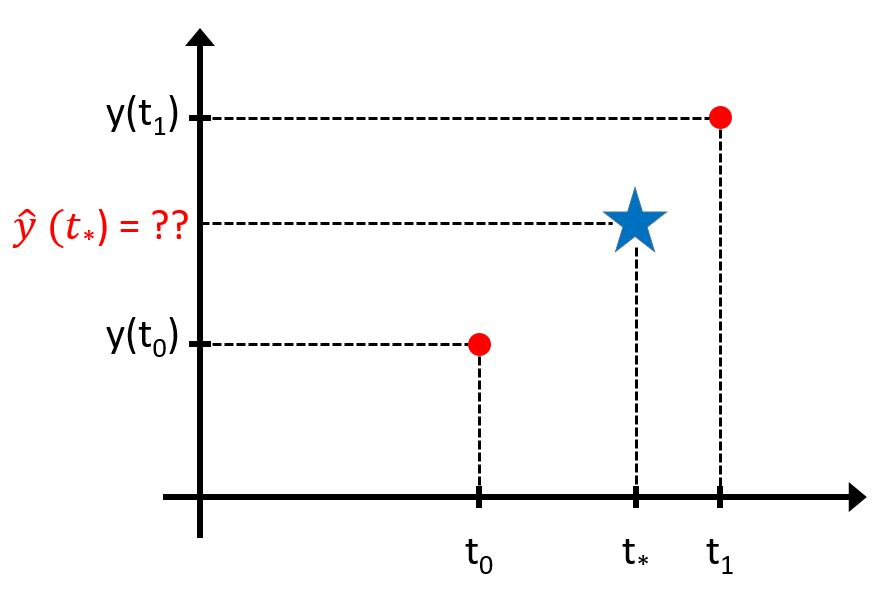
\includegraphics[width=0.8\textwidth]{figures/InterpMeaning}
\end{figure}
\vspace*{-5mm}
\begin{itemize}
	\item[] \textbf{Given:} data points $(t_0,y(t_0))$ \& $(t_1,y(t_1))$ and $t_\star$
	\item[] \textbf{Calculate:} interpolated value $\hat{y}(t_\star)$
\end{itemize}

\end{frame}

%==============================================================

\begin{frame}[fragile]

\frametitle{Linear interpolation}

\vspace*{-5mm}
\begin{figure}[ht]
	\centering
	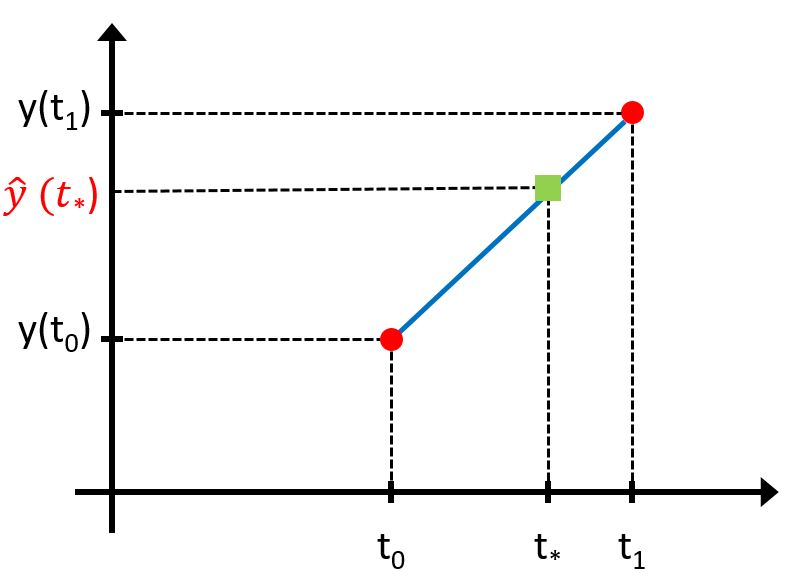
\includegraphics[width=0.7\textwidth]{figures/LinInterpMeaning}
\end{figure}
\vspace*{-5mm}
\begin{itemize}
	\item interpolated value $\hat{y}(t_\star)$ lies on straight line connecting $(t_0,y(t_0))$ \& $(t_1,y(t_1))$
\end{itemize}

\end{frame}

%==============================================================

\begin{frame}[fragile]

\frametitle{Linear interpolation using \texttt{interp1d}}

\begin{itemize}
	\item \texttt{interp1d} function from \texttt{scipy.interpolate}
	\item \texttt{pip install scipy} at console first
	\item call to \texttt{interp1d} returns a function
	\item use the function in console
	\item live demo
\end{itemize}

\end{frame}

%==============================================================

\begin{frame}[fragile]

\frametitle{Linear interpolation in Python}

\texttt{Week6MonLinear.py}

\begin{lstlisting}[style=CStyle,basicstyle=\scriptsize]
import numpy as np
import matplotlib.pyplot as plt
from scipy.interpolate import interp1d

# seed random number generator to reproduce lecture results
np.random.seed(27101967)

N = 11
t = np.linspace(0,100,11)           # 0,10,20,...,100
tnew = np.linspace(0,100,100*N)     # 0,0.1,0.2,...,100
n = np.random.uniform(-25,25,N)     # noise on linear function

m = 3                               # gradient
b = 50                              # intercept
y = m*t + b + n                # dataset is straight line + noise
\end{lstlisting}
\end{frame}

%==============================================================

\begin{frame}[fragile]

\frametitle{Linear interpolation in Python (ctd.)}

\begin{lstlisting}[style=CStyle,basicstyle=\scriptsize]
# INTERPOLATION
f = interp1d(t, y)

# PLOT RESULTS
plt.plot(t, y, 'ro')
plt.xlabel('t')
plt.ylabel('y(t)')
plt.plot(tnew, f(tnew), 'b')
plt.title('Linear interpolation')
plt.show()
\end{lstlisting}
\end{frame}

%==============================================================

\begin{frame}[fragile]

\frametitle{Linear interpolation}

\vspace*{-3mm}
\begin{figure}[ht]
	\centering
	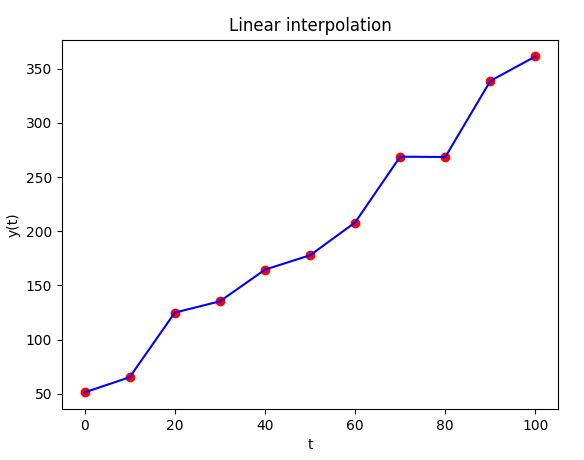
\includegraphics[width=0.7\textwidth]{figures/Week6MonLinearInterp}
\end{figure}
\vspace*{-5mm}
\begin{itemize}
	\item ``stitches together'' straight line segments
\end{itemize}

\end{frame}

%==============================================================

\begin{frame}[fragile]

\frametitle{Beyond linear interpolation}

%The problem with this approach is that the slopes of adjacent lines change abruptly at each data-point –called as C1discontinuity.
%•This can be resolved by stitching piecewise quadratic polynomials between consecutive point pairs and requiring that
%Adjacent polynomials actually pass through the point (interpolatorycondition)
%Adjacent polynomials have the same slope at that point (C1continuity condition)
%
%We could go one step further and require that
%Adjacent polynomials have the same second derivative at that point (C2continuity condition)
%•This requires that the polynomials be piecewise cubic(degree 3) at least.
%•This type of interpolation is called cubic-splineinterpolationand is very popular in graphics and image processing.
%•The data-points (where the continuity conditions) are imposed are called as knotsor control points.
%•A cubic splineis a piecewise polynomial that is twice continuously differentiable (including at the knots).

\begin{itemize}
	\item[] \textbf{Problem:} slopes of adjacent \blue{straight lines} change abruptly at \red{data points}
\end{itemize}

\end{frame}

%==============================================================

\begin{frame}[fragile]

\frametitle{Cubic splines}

\begin{itemize}
	\item degree 1 is linear, degree 2 is parabola, degree 3 is cubic
	\item we're hiding lots of maths here, but we can use Python to implement without needing that maths
	\item maths is interesting!
\end{itemize}

\end{frame}

%==============================================================

\begin{frame}[fragile]

\frametitle{Cubic spline in Python code}

\begin{itemize}
	\item half page code
	\item \texttt{Week6MonCubic.py}
	\item live demo
\end{itemize}

\end{frame}

%==============================================================

\begin{frame}[fragile]

\frametitle{Cubic spline interpolation}

\vspace*{-3mm}
\begin{figure}[ht]
	\centering
	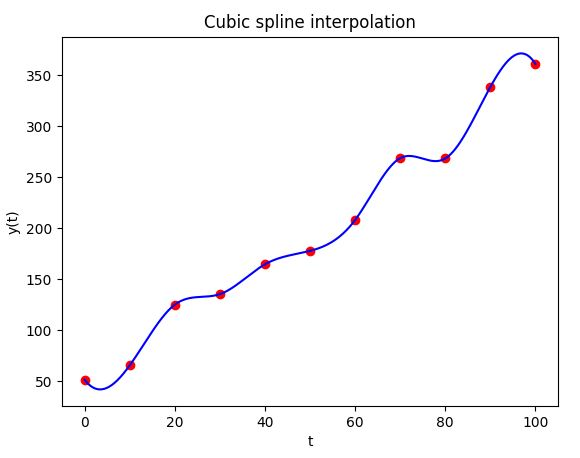
\includegraphics[width=0.7\textwidth]{figures/Week6MonCubicSpline}
\end{figure}
\vspace*{-5mm}
\begin{itemize}
	\item ``stitches together'' \emph{cubic} polynomials
\end{itemize}

\end{frame}

%==============================================================

\begin{frame}[fragile]

\frametitle{$2)$ Assignment 1}

\begin{itemize}
	\item key dates: out, due date for submission
	\item counts for $20$\% of course grade
	\item how assessed: in lab, week 7 (after recess)
	\item the basic ideas behind the lab
	\item this weeks 2-hr face-face lab:
	\begin{itemize}
		\item get started on the assignment
		\item there isn't a week 6 lab sheet: assignment in place of work sheet
	\end{itemize}
\end{itemize}

\end{frame}

%==============================================================

\begin{frame}[fragile]

\frametitle{$3)$ Mid-term quiz}

\begin{itemize}
	\item Thursday 1 April, 4--5pm
	\begin{itemize}
		\item during scheduled lecture time
		\item but there will not be any Zoom or YouTube livestream on 1 April
	\end{itemize}
	\item 40-minute quiz
	\item open-book

	\item quiz will appear on BB at 4:10~pm
	\item counts for $15$\% of course grade
	\item what you'll be asked
\end{itemize}

\end{frame}

%==============================================================

\begin{frame}[fragile]

\frametitle{}

\begin{itemize}
	\item what you can do to prepare for the quiz
	\begin{itemize}
		\item read THIS csv--- can get started now!
		\item you'll be asked to write Python code to do some calculations on a specified column
		\item enter your results into BB
		\item cut-and-paste code into BB
	\end{itemize}
	\item can practice NOW in BB
	\item demo to class in lecture
\end{itemize}

\end{frame}

%==============================================================

\begin{frame}[fragile]

\frametitle{Lecture summary}
\begin{itemize}
	\item Interpolation
	\begin{itemize}
		\item linear interpolation
		\begin{itemize}
			\item straight line ``join the dots''
		\end{itemize}
		\item cubic spline interpolation
		\begin{itemize}
			\item smoothly connects data points
		\end{itemize}
	\end{itemize}

	\item[]
	
	\item Assignment 1
	\begin{itemize}
		\item xxx
	\end{itemize}

	\item[]
	
	\item Mid-term quiz
		\begin{itemize}
			\item xxx
		\end{itemize}
		
\end{itemize}
\end{frame}

\end{document}